\chapter{Contexte réglementaire et modélisation en assurance vie}
\label{chap:contexte}
\newpage
\section{Les spécificités des produits d'assurance vie épargne}
\label{sec:spec_av}

\subsection{Principes fondamentaux du contrat d'assurance vie}

L'assurance vie est une convention par laquelle un assureur, en contrepartie du versement de primes, s'engage à verser un capital ou une rente à la survenance d'un événement incertain lié à la durée de la vie humaine. Cet événement, qui constitue l'aléa au cœur du contrat, peut être le décès de l'assuré avant une date donnée ou, à l'inverse, sa survie jusqu'à cette date. Ce mécanisme repose sur un cycle de production inversé : l'assureur perçoit les primes bien avant de devoir potentiellement régler les prestations, ce qui l'amène à investir ces sommes sur des horizons de temps longs pour honorer ses engagements futurs.

\bigskip

La nature de ces engagements répond à des objectifs variés. Les contrats en cas de vie prévoient le versement d'un capital ou d'une rente à une échéance prévue si l'assuré est en vie ; ils sont typiquement utilisés pour se constituer un complément de retraite ou une épargne de précaution. À l'opposé, les contrats en cas de décès garantissent le versement d'un capital ou d'une rente au(x) bénéficiaire(s) désigné(s) au décès de l'assuré, souvent pour protéger des proches ou anticiper des droits de succession. Il existe également des contrats mixtes qui combinent ces deux garanties.

\bigskip

Le fonctionnement de ces contrats repose sur la capitalisation : les primes versées sont investies pour financer la propre couverture future de l'assuré. De par leur nature, ces engagements s'étendent sur de très longues périodes, conférant au passif de l'assureur une duration élevée, souvent supérieure à huit ans notamment pour des questions de fiscalité.

\bigskip

Une caractéristique fondamentale de l'assurance vie française est sa liquidité. L'assuré dispose de la possibilité de récupérer son épargne à tout moment via un rachat, qui peut être partiel ou total. Cette faculté de rachat constitue une option dont la valeur et le risque doivent être finement gérés par l'assureur, car son exercice a un impact direct sur la duration et les besoins de liquidité du portefeuille. La fiscalité joue un rôle incitatif majeur, les plus-values étant imposées plus lourdement si le rachat intervient avant la huitième année du contrat, encourageant ainsi l'épargne de long terme.

\subsection{Les principaux supports d'investissement}

L'épargne des assurés peut être investie sur deux principaux types de supports aux profils de risque distincts, qui peuvent être combinés au sein de différents types de contrats.

\bigskip


Le \textbf{fonds en euros} est le support historique et sécuritaire de l'assurance vie française. Le risque financier y est intégralement porté par l'assureur, qui s'appuie sur une politique d'investissement prudente, majoritairement orientée vers des actifs obligataires. La sécurité de ce support repose sur un ensemble de garanties contractuelles et réglementaires :
\begin{itemize}
    \item \textbf{La garantie du capital :} C'est la garantie la plus fondamentale. L'assureur garantit à tout moment le capital net investi par l'épargnant. Quelle que soit l'évolution des marchés financiers, la somme initialement versée (nette de frais) ne peut pas diminuer.
    \item \textbf{Le taux technique :} Il s'agit d'un taux de revalorisation minimal garanti sur toute la durée du contrat. Fixé à la souscription, il est aujourd'hui très faible, voire nul, en raison des contraintes réglementaires, mais il a joué un rôle important dans les contrats plus anciens.
    \item \textbf{Le Taux Minimum Garanti (TMG) :} Plus courant aujourd'hui que le taux technique, le TMG est un taux de rendement minimal que l'assureur s'engage à verser pour l'année à venir. Il est fixé annuellement et permet à l'assureur d'ajuster sa politique de rendement.
    \item \textbf{L'effet cliquet :} Ce mécanisme assure que les intérêts générés chaque année sont définitivement acquis. Une fois distribués, ils s'ajoutent au capital garanti et produisent à leur tour des intérêts les années suivantes. Il est impossible de revenir sur les revalorisations passées.
    \item \textbf{La Participation aux Bénéfices (PB) :} L'assureur a l'obligation légale de redistribuer aux assurés une partie significative de ses bénéfices financiers et techniques. Cette participation constitue la majeure partie du rendement annuel, au-delà du TMG. Pour lisser les performances, une partie de cette PB peut être mise en réserve dans une \textit{Provision pour Participation aux Bénéfices} (PPB) que nous appelerons \textit{Provision pour Participations aux Excedents} (PPE) dans la suite de ce mémoire. La PPE doit être reversée aux assurés dans un délai de huit ans au maximum.
\end{itemize}


\bigskip

Les \textbf{unités de compte (UC)} offrent une exposition directe aux marchés financiers. Contrairement au fonds en euros, le risque d'investissement est entièrement porté par l'assuré. L'assureur ne garantit pas la valeur du capital, mais un nombre de parts d'actifs (OPCVM, actions, SCPI, etc.). La valeur de l'épargne fluctue ainsi au gré des marchés, offrant un potentiel de rendement supérieur à long terme, mais exposant également à un risque de perte en capital. Pour l'assureur, ce support est plus simple à gérer car il n'implique pas de garanties financières particulières.

\bigskip

Ces supports sont proposés via deux grandes familles de contrats. Les contrats monosupports permettent d'investir sur un seul type de fonds (soit en euros, soit en UC). Les contrats multisupports sont les plus répandus, quant à eux, combinent au moins un fonds en euros et plusieurs supports en unités de compte, permettant à l'épargnant de répartir son investissement selon son profil de risque. Dans le cadre de cette étude, le portefeuille analysé se compose de contrats multisupports avec une répartition représentative du marché français, soit approximativement 60\% en fonds euros et 40\% en unités de compte.

\subsection{Contexte économique et enjeux actuels}

La gestion de ces produits d'épargne est devenue particulièrement complexe dans l'environnement économique récent. Après une longue période de taux d'intérêt historiquement bas, le secteur de l'assurance a dû s'adapter à un nouveau paradigme marqué par une volatilité accrue et des taux durablement plus élevés.

\bigskip

Cette transition a mis les assureurs en difficulté. Leurs portefeuilles obligataires, constitués en grande partie d'anciennes obligations à faible rendement, présentent une forte inertie. Face à ce stock historique, il leur est difficile de générer des rendements suffisants pour offrir des taux de revalorisation attractifs sur les fonds en euros, capables de concurrencer les nouveaux produits de marché. Cet enjeu de compétitivité, couplé aux exigences de rentabilité et de solvabilité, place la gestion actif-passif au cœur des problématiques actuelles, justifiant pleinement l'introduction du cadre réglementaire qui suit.

\section{Le cadre prudentiel Solvabilité II}
\label{sec:s2}

Entrée en vigueur le 1er janvier 2016, la directive Solvabilité II constitue la norme prudentielle européenne pour la quasi-totalité des assureurs et réassureurs de l'Union Européenne. Son objectif principal est d'harmoniser les pratiques du secteur, d'assurer une protection optimale des assurés et de garantir que les compagnies puissent honorer leurs engagements en toutes circonstances. Pour ce faire, elle instaure une approche économique et prospective, fondée sur une évaluation fine des risques et structurée en trois piliers interdépendants.

\subsection{L'approche stochastique et la valorisation économique}

Un des fondements de Solvabilité II est sa méthode de valorisation des engagements. Pour comprendre la rupture introduite par la norme, il est essentiel de distinguer deux approches complémentaires : déterministe et stochastique.

\begin{itemize}
    \item \textbf{L'approche déterministe} est un outil de pilotage. Elle repose sur une projection unique des variables économiques (courbe des taux, performance des actions, etc.). Bien qu'insuffisante pour la valorisation prudentielle, elle demeure un outil fondamental pour l'assureur. Sa simplicité en fait un instrument privilégié pour l'élaboration du \textit{business plan}, la définition des budgets et la communication d'un scénario central. Elle permet également de réaliser des analyses de sensibilité claires et interprétables. Sa limite principale est son incapacité à valoriser les risques asymétriques.

    \item \textbf{L'approche stochastique} est un outil de valorisation. Pour pallier la limite précédente, cette approche explore un grand nombre de futurs possibles. Elle s'appuie sur un \textbf{Générateur de Scénarios Économiques (GSE)} dont je parlerai plus pleinement dans la fin de ce chapitre. Cet outil sert à produire des ensembles de simulations cohérentes (1000 dans le cadre de cette étude). La valeur d'un indicateur est alors obtenue en calculant la moyenne des résultats sur l'ensemble de ces scénarios, une méthode dite de Monte-Carlo. Cette exploration de multiples futurs est indispensable pour quantifier le coût réel des garanties optionnelles (Taux Minimum Garanti, options de rachat, etc.), qui se matérialise principalement dans les scénarios extrêmes.
\end{itemize}

La différence de valeur entre le résultat de ces deux approches est capturée par le concept de \textbf{TVOG (\textit{Time Value of Options and Guarantees})}. En imposant une approche stochastique, Solvabilité II assure une valorisation \textit{market-consistent}, ou "en juste valeur", des engagements complexes, reflétant le coût réel des options et garanties embarquées dans les contrats.
\subsection{Le Pilier 1 : Exigences quantitatives}

Le Pilier 1 définit les règles de calcul des provisions techniques et du capital de solvabilité. Il introduit la notion de Bilan Prudentiel, une vision économique du bilan comptable où les actifs et les passifs sont évalués de manière cohérente avec leur valeur de marché.

\subsubsection{Le Bilan Prudentiel Solvabilité II}

Le bilan prudentiel se structure de la manière suivante :
\begin{itemize}
    \item \textbf{Les Actifs}, qui sont comptabilisés à leur \textbf{Valeur de Marché (VM)}.
    \item \textbf{Les Provisions Techniques}, qui représentent la valeur des engagements de l'assureur envers ses assurés. Elles se décomposent en deux parties : le \textit{Best Estimate} et la Marge de Risque.
    \item \textbf{Les Fonds Propres Prudentiels}, aussi appelés \textbf{NAV (\textit{Net Asset Value})}, qui constituent la richesse de l'assureur. Ils sont définis par la différence entre la valeur des actifs et celle des engagements : $NAV = VM_{Actifs} - (BE + RM)$.
\end{itemize}

\subsubsection{Les Provisions Techniques (BE et RM)}

Le \textbf{Best Estimate (BE)}, ou \textit{Best Estimate Liability} (BEL), représente la meilleure estimation de la valeur actuelle des flux de trésorerie futurs liés aux engagements d'assurance. Son calcul est réalisé sur un horizon de temps long (40-60 ans) dans l'hypothèse d'un portefeuille en extinction (\textit{run-off}), c'est-à-dire sans l'ajout de nouveaux contrats. Il est obtenu par la moyenne des flux actualisés sur un grand nombre de simulations économiques stochastiques en univers risque neutre~:
\begin{equation}
    BEL = \mathbb{E}^{\mathbb{Q}} \left[ \sum_{j=1}^{T} CF(j) \cdot e^{-\int_0^j r(s)ds} \right] \approx \frac{1}{N}\sum_{i=1}^{N}\sum_{j=1}^{T}\frac{CF_{i}(j)}{(1+r_{i,j})^{j}}
\end{equation}
Où $N$ est le nombre de simulations, $T$ l'horizon de projection, $CF_{i}(j)$ le flux de trésorerie net de l'année $j$ pour la simulation $i$, et $r_{i,j}$ le taux d'actualisation sans risque pertinent. Le BE se subdivise en \textit{Best Estimate Garanti} (BEG) pour les engagements contractuels minimaux et en \textit{Future Discretionary Benefits} (FDB) pour la part de participation aux bénéfices future et discrétionnaire.

\bigskip

La \textbf{Marge de Risque (Risk Margin - RM)} s'ajoute au Best Estimate. Elle correspond au coût qu'un autre assureur exigerait pour reprendre le portefeuille de passif, rémunérant ainsi l'immobilisation du capital nécessaire pour couvrir les risques non-financiers jusqu'à leur extinction. Elle est calculée selon une approche "Coût du Capital" (\textit{Cost of Capital} - CoC) :
\begin{equation}
    RM = \text{CoC}_{\text{rate}} \times \sum_{j=0}^{T} \frac{\text{SCR}_{\text{non-fi}}(j)}{(1+r_{j+1})^{j+1}}
\end{equation}
Où $\text{CoC}_{\text{rate}}$ est le coût du capital (fixé à 6\%), et $\text{SCR}_{\text{non-fi}}(j)$ est la part du SCR couvrant les risques non-financiers à l'année $j$.

\begin{figure}[H]
    \centering
    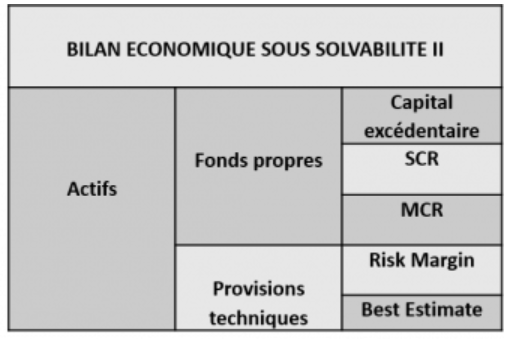
\includegraphics[width=0.65\textwidth]{images/2_chapitres/chapitre1/bilanS2.png}
    \caption{Bilan économique sous Solvabilité II}
    \label{fig:Bilan économique sous Solvabilité II}
\end{figure}


\subsubsection{Les Exigences de Capital (SCR et MCR)}

Solvabilité II définit deux niveaux d'exigence de capital.
\bigskip

Le \textbf{Solvency Capital Requirement (SCR)} est le montant de fonds propres nécessaire pour faire face à une perte inattendue et sévère, calibré pour correspondre à une \textbf{Value-at-Risk (VaR) à 99,5\%}\\ à un horizon d'un an. En cas de non-respect, l'assureur fait l'objet d'un suivi renforcé par le régulateur (l'ACPR en France). En formule standard, son calcul suit une approche modulaire. Pour un risque élémentaire $x$, le SCR est la perte de NAV résultant d'un choc calibré~:
\begin{equation}
    SCR_{x} = NAV_{\text{central}} - NAV_{\text{choc}}
\end{equation}
Pour les risques de passif purs (mortalité, rachat), la formule se simplifie en une variation de Best Estimate ($SCR_{\text{passif}} = \Delta BE$). Les SCR des risques élémentaires sont ensuite agrégés à l'aide de matrices de corrélation pour former le SCR final.

\bigskip

\begin{figure}[H]
    \centering
    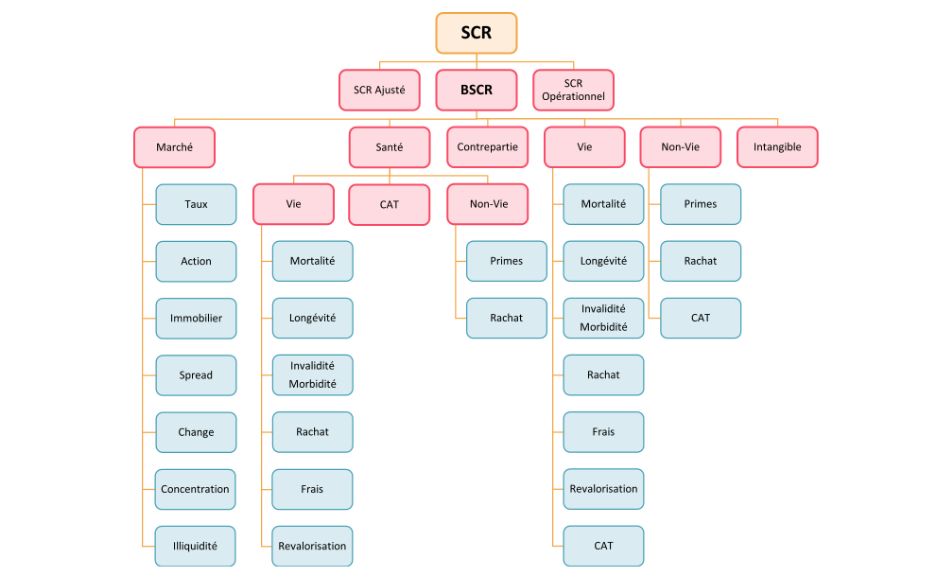
\includegraphics[width=0.95\textwidth]{images/2_chapitres/chapitre1/pieuvre_scr.png}
    \caption{Schéma des modules et sous-modules du SCR en Formule Standard}
    \label{fig:pieuvre_scr}
\end{figure}

Le \textbf{Minimum Capital Requirement (MCR)} est le seuil minimal absolu de fonds propres. Si la NAV de l'assureur tombe en dessous de ce seuil, son agrément peut lui être retiré. Le MCR agit comme un dernier filet de sécurité.




\subsection{Le Pilier 2 : Exigences qualitatives et gouvernance}

Ce pilier se concentre sur la supervision, la gestion des risques et la gouvernance interne. Il impose aux assureurs de mettre en place un \textbf{système de gouvernance} sain, prudent et proportionné. Cela inclut une structure organisationnelle transparente, des politiques écrites claires, et un système de contrôle interne robuste. La direction doit être assurée par au moins deux dirigeants effectifs (\textbf{principe des 4 yeux}) qui doivent répondre à des exigences de compétence et d'honorabilité (\textit{fit and proper}).

\bigskip

Ce système s'articule autour de quatre \textbf{fonctions clés} indépendantes : la fonction actuarielle, la gestion des risques, l'audit interne et la conformité.

\bigskip

L'élément central du Pilier 2 est l'\textbf{ORSA} (\textit{Own Risk and Solvency Assessment}). Il s'agit d'un processus interne par lequel l'assureur évalue, sur un horizon de 3 à 5 ans, l'adéquation entre son profil de risque spécifique, ses limites de tolérance et ses besoins globaux en solvabilité. C'est un outil de pilotage stratégique qui permet d'aller au-delà des hypothèses standards pour refléter la stratégie propre de l'entreprise.
\subsection{Le Pilier 3 : Exigences de reporting et transparence}

Le Pilier 3 vise à assurer la transparence et l'harmonisation de l'information financière à destination du public et des autorités de contrôle. Il définit les rapports et leur fréquence de production (annuelle et trimestrielle).

\bigskip

Les documents clés incluent :
\begin{itemize}
    \item Le \textbf{SFCR} (\textit{Solvency and Financial Condition Report}) : un rapport public annuel sur la solvabilité et la situation financière. Ils ont été particulièrement utiles dans ce mémoire pour illustrer la situation financière des assureurs et avoir des données cohérentes.
        \item Le \textbf{RSR} (\textit{Regular Supervisory Report}) : un rapport narratif détaillé et confidentiel, à destination du superviseur.
        \item Le \textbf{QRT} (\textit{Quantitative Reporting Templates}) : des rapports quantitatifs standardisés remis périodiquement.
        \item Les \textbf{ENS} (\textit{États Nationaux Spécifiques}) : des rapports additionnels demandés par le régulateur local.
        \item Le \textbf{rapport ORSA} : le document confidentiel issu du processus ORSA du Pilier 2.
\end{itemize}

\section{Les Générateurs de Scénarios Économiques (GSE)}
\label{sec:gse}

Le Générateur de Scénarios Économiques (GSE) est un outil mathématique central dans la modélisation stochastique. Il a pour fonction de simuler de multiples trajectoires futures pour les principales variables financières (taux d'intérêt, performance des actions, inflation, etc.). La qualité des projections ALM dépendant directement de la robustesse du GSE, il est nécessaire de distinguer deux cadres de modélisation qui coexistent.

Bien que ces deux univers soient complémentaires, la réglementation Solvabilité II assigne à chacun un rôle très précis pour le calcul des différents indicateurs prudentiels. Le tableau suivant synthétise cette répartition des tâches.

\begin{table}[H]
\centering
\caption{Répartition des calculs Solvabilité II par univers de projection}
\label{tab:s2_par_univers}
\begin{tabularx}{\textwidth}{>{\raggedright\arraybackslash}X >{\raggedright\arraybackslash}X}
\toprule
\textbf{\texorpdfstring{Univers Risque Neutre (Q)}{Univers Risque Neutre (Q)}} & \textbf{\texorpdfstring{Univers Monde Réel (P)}{Univers Monde Réel (P)}} \\
\midrule
\textbf{Indicateurs du Pilier 1 :}
\begin{itemize}[itemsep=2pt]
\item Best Estimate Liability (BEL)
\item Marge de Risque (RM)
\item Solvency Capital Requirement (SCR)
\item Bilan Prudentiel et NAV
\end{itemize}
&
\textbf{Exercices du Pilier 2 :}
\begin{itemize}[itemsep=2pt]
\item ORSA (Own Risk and Solvency Assessment)
\item Business Plan et planification stratégique
\item Test de la pérennité du modèle
\end{itemize} \\
\addlinespace
\textbf{Finalité : Valorisation} \textit{Market-Consistent} à un instant t.
&
\textbf{Finalité : Pilotage} stratégique et prospectif. \\
\bottomrule
\end{tabularx}
\end{table}

La distinction entre ces deux approches est donc fondamentale : l'une sert à valoriser, l'autre à piloter. Les sections suivantes détaillent les modèles mathématiques sous-jacents à chaque univers.

\subsection{\texorpdfstring{L'univers Risque Neutre ($\mathbb{Q}$)}{L'univers Risque Neutre (Q)} : un cadre pour la valorisation}

L'\textbf{univers Risque Neutre ($\mathbb{Q}$)} est un cadre de valorisation théorique, requis par Solvabilité II pour les calculs \textit{market-consistent}. Son objectif n'est pas de prédire l'évolution réelle des marchés, mais de calculer la valeur « juste » d'un actif ou d'un passif à la date de calcul, en se fondant sur les prix de marché observés. Dans cet univers, on postule que tous les investisseurs sont indifférents au risque, ce qui implique que le rendement espéré de n'importe quel actif est égal au taux d'intérêt sans risque. Cette construction, fondée sur l'absence d'opportunité d'arbitrage, est indispensable pour valoriser de manière cohérente les options et garanties complexes des contrats d'assurance. La valeur $V_0$ d'un flux de trésorerie futur $CF_T$ est alors son espérance mathématique sous cette probabilité risque neutre, actualisée au taux sans risque $r(s)$ :
\begin{equation}
    V_0 = \mathbb{E}^{\mathbb{Q}} \left[ CF_T \cdot e^{-\int_0^T r(s)ds} \right]
    \label{eq:valeur_risque_neutre}
\end{equation}
Cet univers constitue le fondement du Pilier 1 de Solvabilité II, utilisé pour le calcul du Best Estimate Liability (BEL) et du Solvency Capital Requirement (SCR).

\subsubsection{Modélisation des taux d'intérêt : le modèle de Hull \& White}
Pour les taux d'intérêt, le modèle de \textbf{Hull \& White à un facteur} est une référence dans le cadre réglementaire. Son principal avantage est sa capacité à se calibrer parfaitement à la courbe des taux sans risque initiale, telle que fournie par l'EIOPA.
\begin{figure}[H]
    \centering
    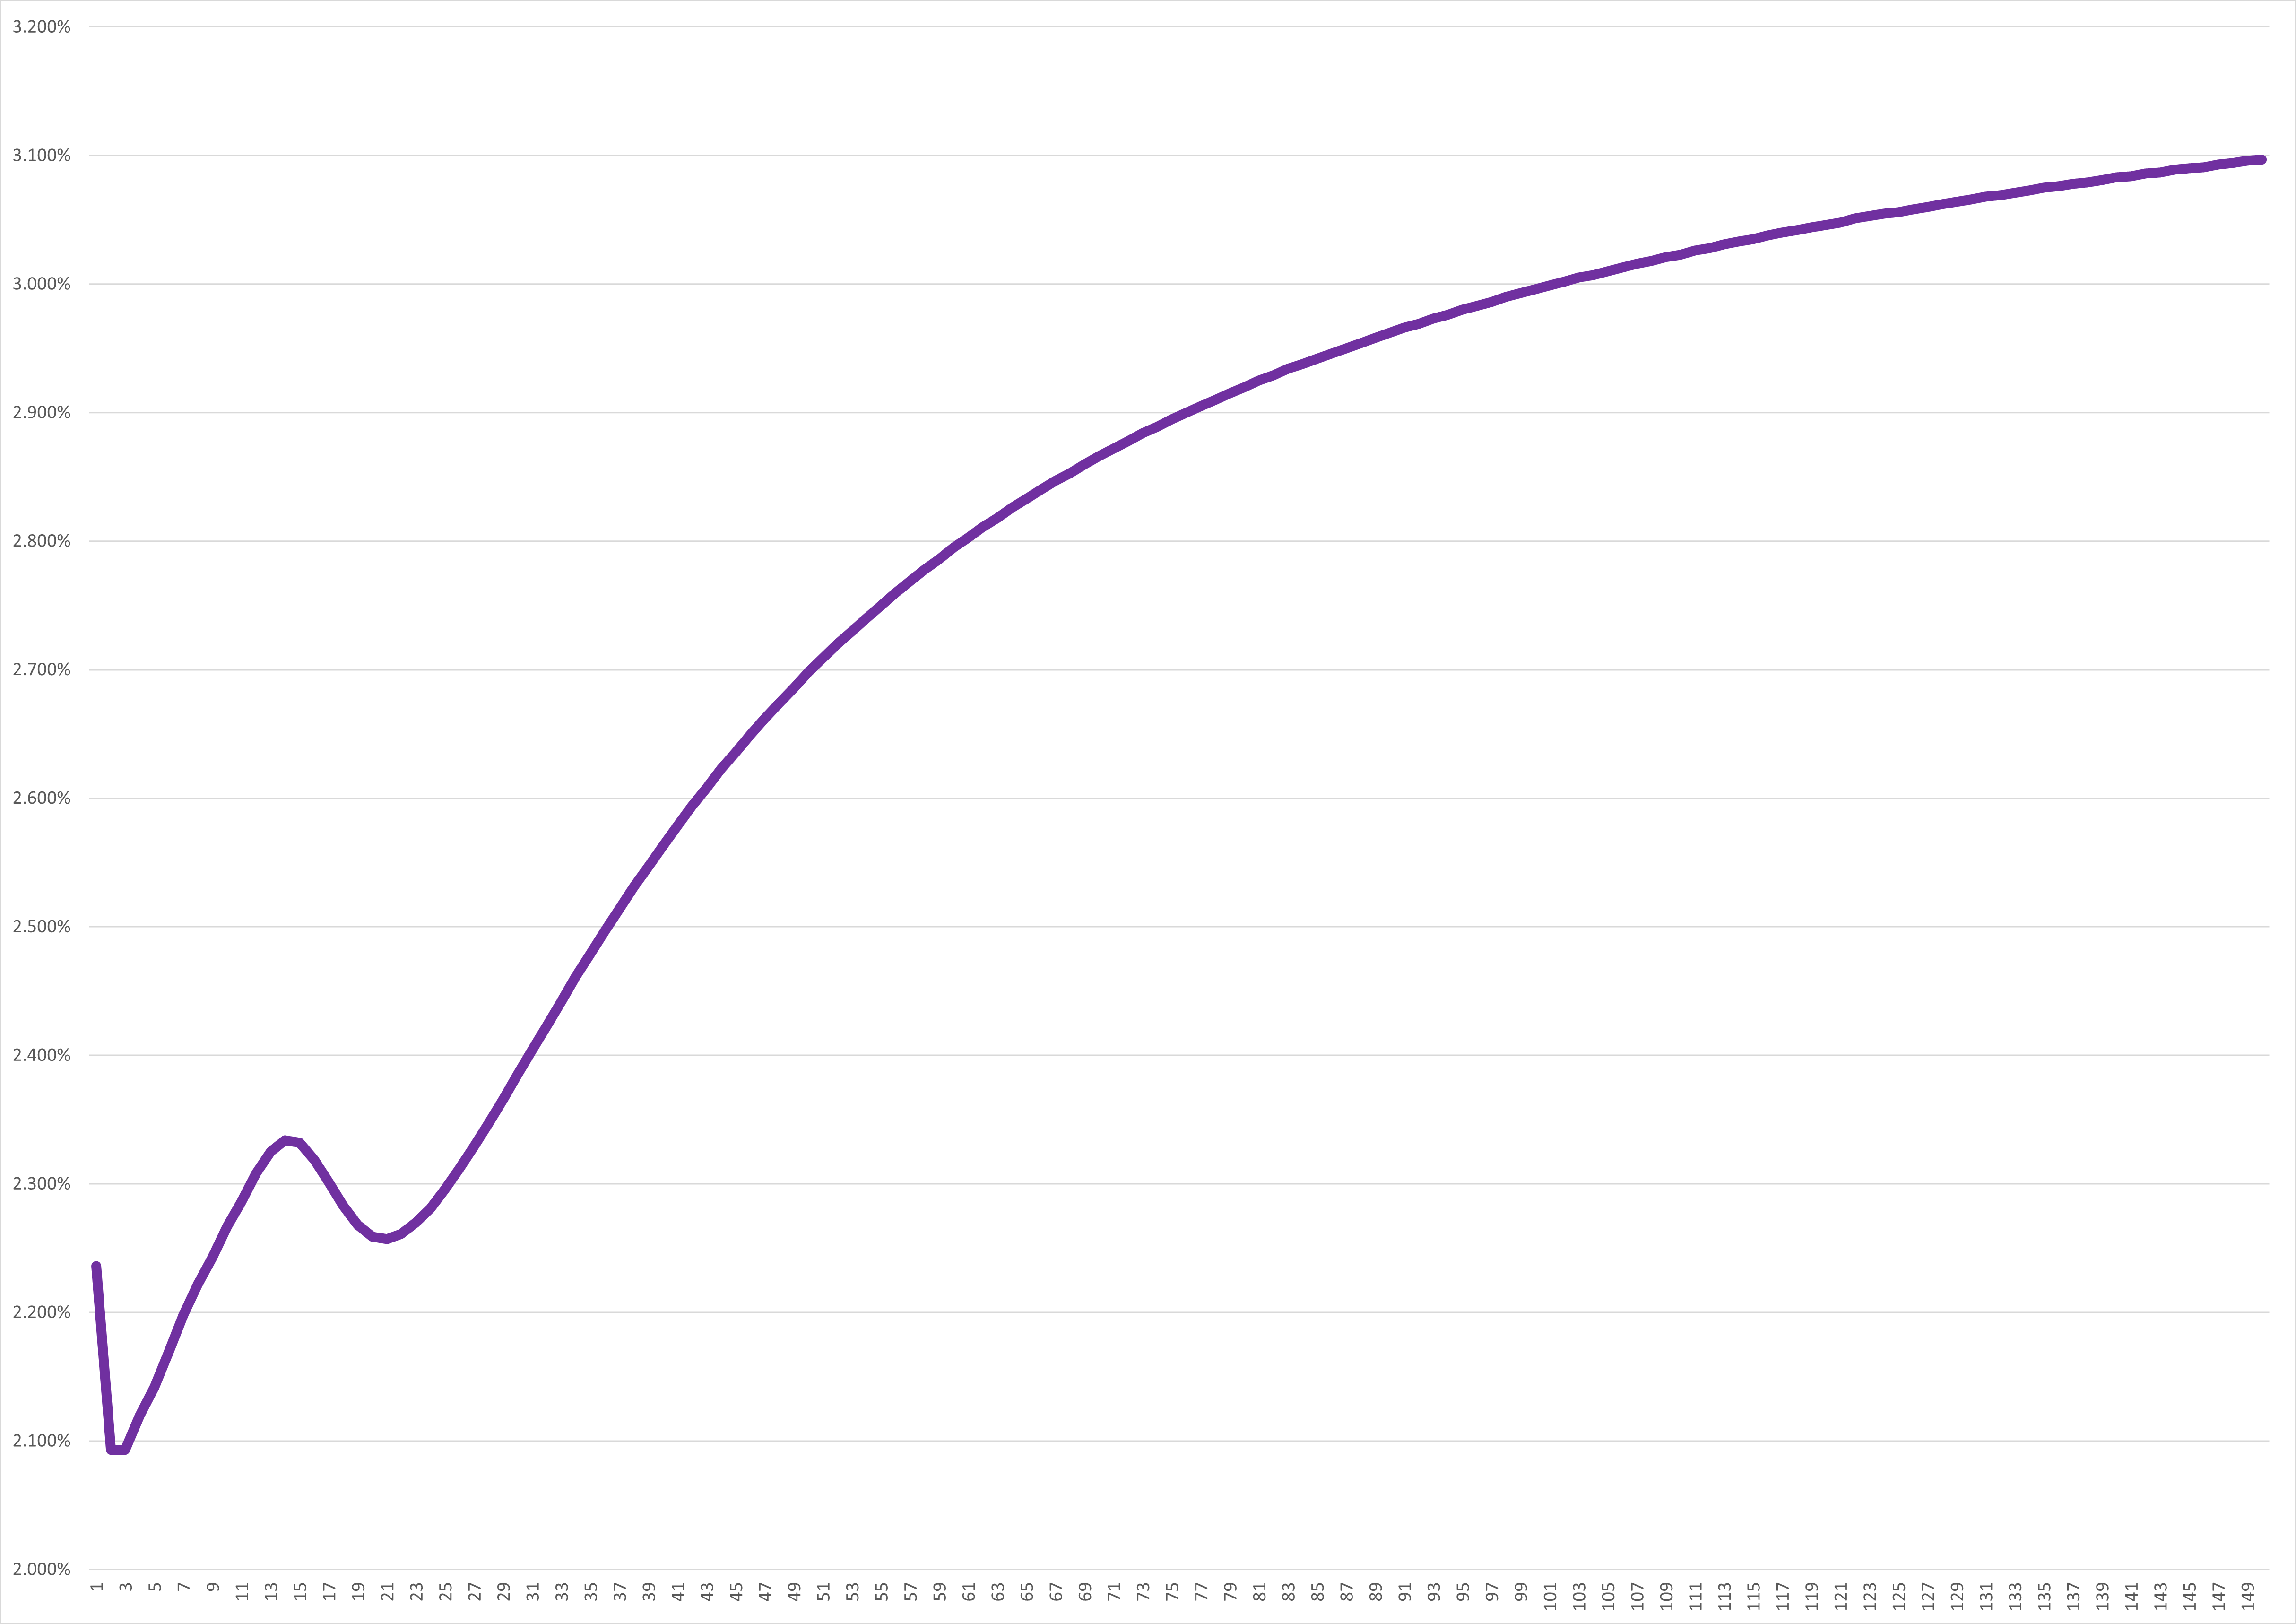
\includegraphics[width=0.65\textwidth]{images/2_chapitres/chapitre1/courbe_EIOPA.png}
    \caption{Courbe des taux sans risque sans \textit{Volatility Adjustment} au 31/12/2024 publiée par l'EIOPA}
    \label{fig:courbe_EIOPA}
\end{figure}

Cette flexibilité est obtenue grâce à un paramètre de retour à la moyenne $\theta(t)$ qui dépend du temps. Son équation différentielle stochastique (EDS) s'écrit :
\begin{equation}
    dr_t = (\theta(t) - ar_t)dt + \sigma dW^{\mathbb{Q}}_t
    \label{eq:hull_white}
\end{equation}
où $r_t$ est le taux d’intérêt court, $a$ la vitesse de retour à la moyenne, $\sigma$ la volatilité et $W^{\mathbb{Q}}_t$ un mouvement brownien sous la mesure risque neutre. Pour des raisons de calcul, nous utilisons la solution discrète de cette EDS :
\begin{equation}
    r_{t+h} = r_t e^{-ah} + \theta(t+h) - \theta(t)e^{-ah} + \sigma \sqrt{\frac{1 - e^{-2ah}}{2a}} Z
    \label{eq:hull_white_discrete}
\end{equation}

\subsubsection{Modélisation des actions et de l'immobilier : le modèle de Black \& Scholes}
Pour les actifs risqués comme les actions ou l'immobilier, le modèle de \textbf{Black \& Scholes} est couramment utilisé. Conformément à la logique risque neutre, le rendement espéré (la dérive du processus) est le taux sans risque $r_t$. L'EDS du prix de l'actif $S_t$ est :
\begin{equation}
    dS_t = r_t S_t dt + \sigma S_t dW^{\mathbb{Q}}_t
    \label{eq:black_scholes_q}
\end{equation}
où $S_t$ est le prix de l'actif, $r_t$ le taux sans risque et $\sigma$ la volatilité de l'actif. La solution de cette EDS est donnée par :
\begin{equation}
    S_t = S_0 \exp\left( \int_0^t \left(r_s - \frac{\sigma^2}{2}\right)ds + \int_0^t \sigma dW^{\mathbb{Q}}_s \right)
\end{equation}
En pratique, on utilise sa solution discrétisée pour simuler les trajectoires de prix sur un pas de temps $h$ :
\begin{equation}
    S_{t+h} = S_t \exp\left( \left(r_t - \frac{\sigma^2}{2}\right)h + \sigma\sqrt{h}Z \right)
    \label{eq:black_scholes_q_discrete}
\end{equation}
où $Z$ est une variable aléatoire suivant une loi normale centrée réduite $\mathcal{N}(0,1)$.

\subsection{\texorpdfstring{L'univers Monde Réel ($\mathbb{P}$)}{L'univers Monde Réel (P)} : un outil de pilotage stratégique}

À l'inverse, l'\textbf{univers Monde Réel ($\mathbb{P}$)} vise à générer des scénarios réalistes pour refléter une évolution plausible des marchés. Son objectif est la projection et la planification stratégique, notamment pour l'exercice ORSA (Pilier 2) ou l'optimisation de l'allocation d'actifs. La différence fondamentale avec l'univers risque neutre réside dans l'introduction d'une prime de risque pour rémunérer la volatilité supportée par les investisseurs. Le rendement espéré d'un actif risqué est donc supérieur au taux sans risque :
\begin{equation}
    \mathbb{E}^{\mathbb{P}}[\text{Rendement de l'actif}] = \text{Taux sans risque} + \text{Prime de risque}
\end{equation}
Cette prime est calibrée à partir d'analyses prospectives, de données historiques et de d'avis d'expert sur le marché.

\subsubsection{Modélisation des taux d'intérêt : le modèle de Vasicek}
Dans l'univers monde réel, le modèle de \textbf{Vasicek} est souvent préféré pour sa parcimonie et son interprétation économique. Il modélise un retour des taux courts $r_t$ vers une moyenne de long terme constante $b$, ce qui correspond à une vision économique plus stable. Son EDS est :
\begin{equation}
    dr_t = a(b - r_t)dt + \sigma dW^{\mathbb{P}}_t
    \label{eq:vasicek}
\end{equation}
où $a$ est la vitesse de retour à la moyenne, $b$ la moyenne de long terme du taux, $\sigma$ sa volatilité et $W^{\mathbb{P}}_t$ un mouvement brownien sous la mesure monde réel. La solution de cette EDS est :
\begin{equation}
    r_t = r_0 e^{-at} + b(1-e^{-at}) + \sigma \int_0^t e^{-a(t-s)}dW^{\mathbb{P}}_s
\end{equation}
Pour calibrer ces modèles, les données choisies en entrée sont typiquement des séries temporelles historiques : Euribor 3 mois pour les taux courts, l'indice des OAT 10 ans pour les taux longs, les cotations de l'IEIF pour l'immobilier et l'EuroStoxx pour les actions.

\subsubsection{Modélisation des actions et de l'immobilier : le modèle de Black \& Scholes avec prime de risque}
Le modèle de Black \& Scholes est également utilisé, mais sa dérive est modifiée pour inclure la prime de risque. Le rendement espéré $\mu$ est désormais une constante supérieure au taux sans risque moyen : $\mu > r$. L'EDS devient :
\begin{equation}
    dS_t = \mu S_t dt + \sigma S_t dW^{\mathbb{P}}_t
    \label{eq:black_scholes_p}
\end{equation}
La solution de cette EDS est le fameux mouvement brownien géométrique :
\begin{equation}
    S_t = S_0 \exp\left( \left(\mu - \frac{\sigma^2}{2}\right)t + \sigma W^{\mathbb{P}}_t \right)
\end{equation}

\subsection{Synthèse des deux univers}

Le tableau suivant résume les caractéristiques et les usages des deux univers de projection. Si l'univers risque neutre $\mathbb{Q}$ répond à la question « \textit{Combien vaut cet engagement aujourd'hui ?} », l'univers monde réel $\mathbb{P}$ répond à « \textit{Quelle sera ma situation financière demain ?} ».

\begin{table}[H]
    \centering
    \caption{Synthèse comparative des univers de projection}
    \label{tab:univers_s2_comp}
    \begin{tabularx}{\textwidth}{l >{\raggedright\arraybackslash}X >{\raggedright\arraybackslash}X}
        \toprule
        \textbf{Critère} & \textbf{\texorpdfstring{Univers Risque Neutre ($\mathbb{Q}$)}{Univers Risque Neutre (Q)}} & \textbf{\texorpdfstring{Univers Monde Réel ($\mathbb{P}$)}{Univers Monde Réel (P)}} \\
        \midrule
        \textbf{Objectif}
        &
        \textbf{Valorisation} \textit{Market-Consistent} (Pilier 1 : BEL, SCR). Calculer une valeur juste à $t=0$.
        &
        \textbf{Projection} stratégique (Pilier 2 : ORSA, Business Plan). Simuler des futurs plausibles. \\
        \addlinespace
        \textbf{Rendement Espéré (Actifs risqués)}
        &
        Taux sans risque ($r_t$). Aucune prime de risque.
        &
        Taux sans risque + Prime de risque ($\mu = r + \text{prime}$). \\
        \addlinespace
        \textbf{Modèle de Taux Typique}
        &
        \textbf{Hull \& White}. Flexible, calibré à la courbe des taux initiale.
        &
        \textbf{Vasicek}. Économique, retour à une moyenne de long terme. \\
        \addlinespace
        \textbf{Calibration}
        &
        Calibré sur les prix des instruments financiers \textbf{actuels} (courbe des taux, volatilités implicites).
        &
        Calibré sur des \textbf{données historiques} et des \textbf{anticipations d'experts} (primes de risque). \\
        \bottomrule
    \end{tabularx}
\end{table}

\section{La gestion Actif-Passif (ALM) : définitions et enjeux}
\label{sec:alm}

La gestion Actif-Passif, ou \textit{Asset-Liability Management} (ALM), est la discipline qui vise à piloter de manière coordonnée l'actif et le passif du bilan d'un assureur. L'enjeu fondamental de l'ALM découle directement du \textbf{cycle de production inversé} : les primes sont collectées et investies bien avant que les prestations ne soient versées. Ce décalage temporel crée une \textbf{inadéquation} (\textit{mismatch}) structurelle entre les caractéristiques des actifs (soumis à la volatilité des marchés) et celles des passifs (de longue durée et parfois assortis de garanties).

\bigskip

L'objectif de l'ALM est donc de gérer activement les risques découlant de cette inadéquation, notamment le \textbf{risque de taux d'intérêt}, le \textbf{risque de liquidité} (lié aux rachats) et les \textbf{risques de marché} (actions, crédit), afin de s'assurer que les flux générés par les actifs seront suffisants pour honorer les engagements, tout en optimisant la rentabilité et en respectant les contraintes réglementaires.

\bigskip

Pour ce faire, les assureurs s'appuient sur des \textbf{modèles ALM} sophistiqués. Ces modèles simulent l'évolution conjointe de l'actif et du passif sur des horizons de temps longs (40 ans ou plus), sous une multitude de scénarios économiques. Ils intègrent les caractéristiques des portefeuilles, les lois de comportement des assurés (rachats, mortalité) et les règles de gestion de l'assureur (politique de PB, stratégie de couverture). Ces projections permettent d'évaluer l'impact de différentes stratégies et constituent un outil indispensable à la prise de décision.

\section{La représentation du passif : le concept de \textit{Model Point}}
\label{sec:mp}

\subsection{La nécessité de l'agrégation}

Les portefeuilles d'assurance vie comptent souvent des centaines de milliers, voire des millions de polices. Une modélisation "police à police" est techniquement possible mais informatiquement irréalisable pour des calculs stochastiques complexes comme ceux requis par les modèles ALM. La charge de calcul deviendrait prohibitive. La simplification du portefeuille de passif n'est donc pas un choix, mais une contrainte opérationnelle fondamentale.

\bigskip

La réponse standard à cette contrainte est la création de \textbf{\textit{Model Points}} (MP). Un MP est un contrat synthétique représentant un agrégat de polices partageant des caractéristiques homogènes. L'objectif est de réduire drastiquement le volume de données à traiter tout en préservant les propriétés actuarielles et financières essentielles du portefeuille complet. La qualité de la représentation dépend directement de la pertinence des critères de regroupement (caractéristiques du produit, de l'assuré, du contrat), souvent optimisés par des techniques de classification statistique (\textit{clustering}).

\subsection{Du Model Point à la problématique du mémoire}

L'utilisation des \textit{Model Points} constitue la méthode standard pour agréger le passif et rendre les modèles ALM opérationnels. Cependant, la manière dont ces groupes de contrats sont formés à partir des polices individuelles a un impact direct et significatif sur la valorisation des indicateurs réglementaires et leur sensibilité aux chocs.

\bigskip

La problématique centrale de ce mémoire est donc d'optimiser cette étape fondamentale de l'agrégation. En partant du portefeuille granulaire "police à police", nous cherchons à définir, comparer et tester différentes méthodes de regroupement pour créer des \textit{Model Points}. L'objectif est de construire une méthodologie de simplification optimale, c'est-à-dire celle qui minimise l'erreur d'agrégation tout en garantissant la plus grande stabilité des indicateurs Solvabilité II (SCR, Marge de Risque, NAV) lors du calcul des différentes sensibilités. Cette section introductive pose donc les fondations de notre analyse : la simplification étant une nécessité, comment s'assurer que la méthode de regroupement choisie est la plus fidèle et la plus robuste possible ?
